\documentclass[tikz,border=2pt]{standalone}
\usepackage{amsmath}
\usepackage{pgfplots}
\pgfplotsset{compat=1.18}

\begin{document}
% Lower sum (rectangles under the graph) and upper sum (rectangles over it) for one partition:
% the integral is the common value they squeeze towards when the partition is refined.
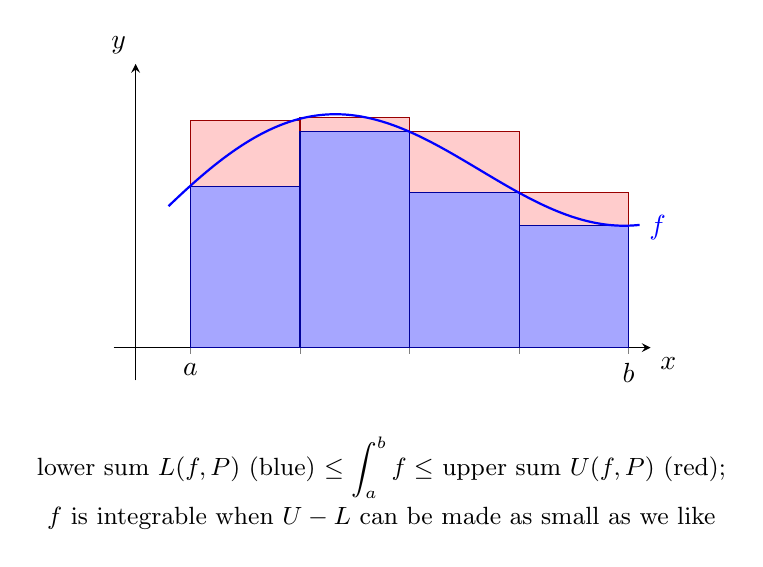
\begin{tikzpicture}
	\begin{axis}[
		axis lines=middle,
		xmin=-0.2, xmax=4.7,
		ymin=-0.3, ymax=2.6,
		xtick={0.5,1.5,2.5,3.5,4.5}, xticklabels={$a$,,,,$b$},
		ytick=\empty,
		xlabel={$x$}, ylabel={$y$},
		xlabel style={below right}, ylabel style={above left},
		samples=150, smooth, clip=false,
		width=8.4cm, height=5.6cm
		]
		% f(x)=1+0.8 sin(x)+0.2x on [0.5,4.5]; piecewise sup/inf approximated at endpoints/interior
		% upper rectangles (max on each piece), drawn first
		\fill[red!20, draw=red!60!black] (axis cs:0.5,0) rectangle (axis cs:1.5,2.08);
		\fill[red!20, draw=red!60!black] (axis cs:1.5,0) rectangle (axis cs:2.5,2.11);
		\fill[red!20, draw=red!60!black] (axis cs:2.5,0) rectangle (axis cs:3.5,1.98);
		\fill[red!20, draw=red!60!black] (axis cs:3.5,0) rectangle (axis cs:4.5,1.42);
		% lower rectangles (min on each piece)
		\fill[blue!35, draw=blue!60!black] (axis cs:0.5,0) rectangle (axis cs:1.5,1.48);
		\fill[blue!35, draw=blue!60!black] (axis cs:1.5,0) rectangle (axis cs:2.5,1.98);
		\fill[blue!35, draw=blue!60!black] (axis cs:2.5,0) rectangle (axis cs:3.5,1.42);
		\fill[blue!35, draw=blue!60!black] (axis cs:3.5,0) rectangle (axis cs:4.5,1.12);
		\addplot[thick, blue, domain=0.3:4.6] {1+0.8*sin(deg(x))+0.2*x};
		\node[blue, anchor=west] at (axis cs:4.6,1.1) {$f$};
	\end{axis}
	\node[anchor=north, align=center, font=\small] at (3.4,-0.6) {lower sum $L(f,P)$ (blue) $\le\displaystyle\int_a^b f\le$ upper sum $U(f,P)$ (red);\\[2pt] $f$ is integrable when $U-L$ can be made as small as we like};
\end{tikzpicture}
\end{document}
